\chapter{Metodología}

\section{Procesos}
Al momento de iniciar cualquier proyecto de desarrollo de software, hay que tener en cuenta dos factores relevantes, el primer factor el hardware, depende en esencia de la elección del grupo de desarrollo y además de la calidad y forma de usar el mismo, el segundo factor el software, es un aspecto algo mas complejo, principalmente por los siguientes factores:
\begin{itemize}
	\item El sistema en muchas ocasiones no llenan las expectativas del usuario, no solo en su parte visual sino además de su parte funcional
	\item Según la metodología adoptada por el desarrollador o desarrolladores, el sistema suele tener "caídas" en diferentes ocasiones, lo que hace que para el usuario final sea una verdadera molestia
	\item Conocer el costo exacto del desarrollo de cualquier software es una tarea difícil de realizar además que se da con poco éxito, básicamente por las dificultades y pormenores que se pueden generar en el proceso.
	
\end{itemize}
\subsection{Proceso en Espiral}
En 1988 y gracias a el esfuerzo de Barry Boen nace "El modelo evolutivo espiral", como respuesta a todas estas necesidades que implica el desarrollo de software, la gran ventaja de este modelo es que permite evaluar cada posible riesgo y evalúa las posibles alternativas para generar un software mucho mas robusto. El mecanismo que usa esta metodología es principalmente diferentes ciclos hasta que el software diseñado sea aceptado y no necesite mejorarse con un nuevo ciclo.

El modo espiral tiene como objetivo cubrir las necesidades tanto de desarrolladores como de el usuario, en cuanto a posibles cambios que se deban hacer por cualquier motivo, es por esto que tan pronto culmina un proceso de desarrollo, simplemente se considera el punto de partida para un nuevo ciclo de constantes mejores, por ello este modelo maneja 4 pasos principales:

\begin{enumerate}
	\item Determinar los objetivos
	Este paso consiste en fijarse las metas que hay que alcanzar para luego de ello identificar las limitaciones que puede llegar a tener el objetivo planteado, ademas de ello cada objetivo tiene su gestión propia y sus riesgos propios que también deben ser sometidos a una análisis.
	\item Análisis de riesgo
	Debido a que el primer paso permite evidenciar los riesgos posibles de el objetivo en el que se esté trabajando, es obligación entonces en este paso hacer un análisis detallado de cada uno de ellos, además de planear estrategias para resolver los mismos.
	\item Desarrollar, verificar y validar
	Gracias a los primeros dos pasos, es posible escoger de manera apropiada el paradigma que se usara para desarrollar el ciclo afrontado.
	\item Planificar 
	En este paso, es donde se decide si en realidad se necesita otro ciclo adicional para alcanzar el objetivo principal, en este caso el desarrollo de el software con todos los requerimientos y funcionalidades, es por ello que cada ciclo crea una nueva versión de lo que se va trabajando.
\end{enumerate}

\begin{figure}[h!]
	\centering
	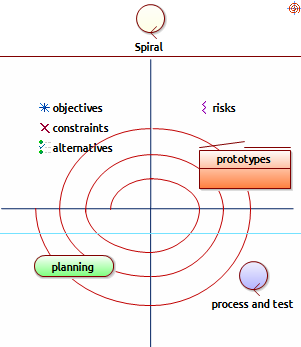
\includegraphics[width=0.7\linewidth]{proyecto/imgs/procesoEspiral}
	\caption{Proceso en Espiral}
	\label{fig:procesoespiral}
\end{figure}

Este método tiene una característica distintiva de los demás métodos y es principalmente la evaluación de riesgos, el riesgo es todo para este, debido a que el riesgo es la diferencia entre una implementación limpia, a otra que pueda ser mas compleja, y genere sobre costos en el proyecto.
\newpage 
\subsection{Proceso de modelo en V}
Por otro lado, el modelo en V es un proceso ampliamente aceptado para el ciclo de vida y desarrollo del software. Es uno de los mejores modelos para software ya que impulsa las pruebas y los test. Cada etapa de este modelo tiene dos objetivos : uno es la validación y el segundo es la verificación. \cite{7062536}
\\
En el presente proyecto, se asume la validación como identificar
los  riesgos y verificación como seguimiento o evaluación de los requerimientos.Las ventajas que proporciona trabajar con este proceso son : 

\begin{itemize}
	\item El modelo en V hace más explicita la tarea parte de la iteración de las actividades del proceso.
	\item Las pruebas de cada fase ayudaran a corregir posibles errores sin tener que esperar a que sean rectificados en la etapa final del proceso.
	\item Con las pruebas unitarias y de integración se consigue obtener exactitud en los programas.
\end{itemize}

\begin{figure}[h!]
	\centering
	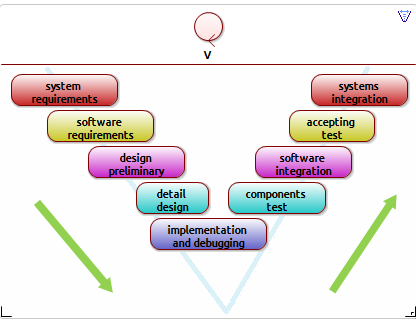
\includegraphics[width=0.7\linewidth]{proyecto/imgs/modeloV}
	\caption{Diagrama del proceso en V}
	\label{fig:modelov}
\end{figure}


\section{Metodologías Ágiles}
La elección de una metodología en el proyecto es importante dado que ayuda a explicar cómo funciona el equipo de trabajo, facilita la comprensión de las responsabilidades y las prioridades. En adición, es vital para medir y mostrar el progreso en el desarrollo de software y lo más importante que provee es un marco de aprendizaje constante para los participantes.
Es por eso que a continuación se hablará en detalle de la metodología seleccionada para la situación problema del presente.\\
\subsection{Crystal }
Crystal es una familia creada por Alistair Cockborn, uno de los fundadores del Manifiesto Agil.El nombre "Crystal" viene de la caracterización de dos dimensiones en los proyectos : tamaño y criticidad \cite{cockburn2004crystal} . Estas dos dimensiones fueron relacionadas con el color y la dureza de los cristales. \\ Por ejemplo , los proyectos de mayor complejidad son los de un cristal con un color más oscuro, ya que necesitan una metodología más firme, con más validación y reglas de verificación.
Comparten tres postulados que son :
\begin{itemize}
	\item Entregas frecuentes
	\item Comunicación cercana
	\item Mejora reflexiva
\end{itemize}

Lo cierto es que no existe en concreto una sola metodología llamada Crystal, hay diferentes metodologías y depende del proyecto que se vaya a desarrollar para seleccionar la más apropiada. En este caso,se escoge la metodología \emph{Crystal Clear}.\\

\begin{figure}[h!]
	\centering
	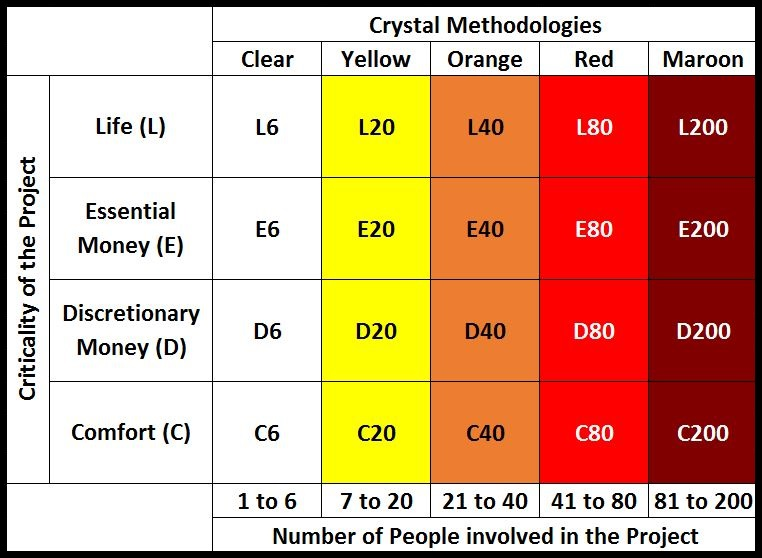
\includegraphics[width=0.7\linewidth]{proyecto/imgs/crystalM}
	\caption{Metodologías Crystal}
	\label{fig:crystalm}
\end{figure}


\subsection{Crystal Clear}
Crystal Clear es un derivado de Crystal que se puede adoptar cuando el equipo de trabajo es pequeño (de dos a ocho personas) que y que comparten o trabajan en el mismo sitio u oficina. Se fortalece lo que es la comunicación estrecha, se puede conversar sobre las prioridades del proyecto, el estado, los requisitos y el diseño a diario. Como primera tarea para la adopción de esta metodologia se tiene que resaltar los puntos fuertes y las debilidades de la organización o del equipo de trabajo y se deben seguir las recomendaciones de la metodología para potenciar las fortalezas y cubrir o contrarrestar las debilidades. \\

Para profundizar más en esta metodología, se describirá a grandes rasgos cada una de las 7 propiedades que tiene Crystal Clear.

\subsubsection{Entregas Frecuentes}
Si se hacen entregas constantes los patrocinadores obtienen una retroalimentación crítica sobre la tasa de progreso del equipo. Los clientes tienen una oportunidad de descubrir si sus peticiones originales se cumplieron o si necesitan ser redefinidas. Es beneficioso para el equipo porque permite que los proceso se depuren, se desarrollen y se implementen, en el fondo el impulso moral incrementa a traves de los logros.\\

Por lo general estas entregas son recomendables en periodos semanales (si se despliegan en la web) o máximo dos meses. En contraste con lo anterior, no siempre se encuentran los usuarios que se acomoden a las entregas tan seguidas, esto puede resultar un contra ya que algunas fallas se pueden pasar por alto sin la aprobación del cliente. Se propone entonces que se busque un usuario amigable y que no tenga problema con testear y probar el programa así sólo sea por curiosidad, de esta manera por lo menos se tiene una fuente que proveerá consejos, indicaciones y posibles mejoras para el producto.

\subsubsection{Mejora Reflectiva}
Una de las mejores características de esta metodología es la posibilidad de convertir las fallas y los errores en un éxito. Esto se hace a través de la reflexión, metaforicamente es como mirarse en un espejo y reconocer las cosas que no están funcionando pero en simultaneo poder mirar lo que tambien funciona, con el objetivo de cambiar lo que no funciona en la próxima iteración. Este proceso no toma mucho tiempo.\\

Lo mejor sería que esto se hiciera cada pocas semanas, una vez al mes, o dos veces por ciclo de entrega, se programan y se reunen en un taller de reflexión o retrospectiva de la iteración para discutir cómo están funcionando las cosas. Aqui se discute lo que permanecerá y lo que cambiará para el próximo periodo. 

\subsubsection{Comunicación Osmótica}
Esto consiste en que la información fluye en todos los miembros del equipo y que a su vez deberia recogerse esa información relevante como si se estuviera haciendo ósmosis\footnote{La ósmosis es un fenómeno en el que se produce el paso o difusión de un disolvente a través de una membrana semipermeable (que permite el paso de disolventes, pero no de solutos), desde una disolución más diluida a otra más concentrada.}. Esto se logra si todos se encuentran en la misma habitación, si alguien hace una pregunta, otros en la sala se pueden "sintonizar" contribuyendo a la discusión.\\

Esta forma de comunicación hace que el costo sea bajo y que los errores sean corregidos rápidamente y que el conocimiento se expanda de esta misma manera. Se corrigen y se obtienen nuevas propuestaas antes de hacer que los errores pequeños existentes crezcan.

\subsubsection{Seguridad Personal}
La seguridad personal es la capacidad de hablar cuando algo molesta, no cuadra o no compartes con los otros sin el miedo a represalias. Esto implica desde charlas con el gerente o lider del proyecto manifestando inconvenientes con el horario o tambien con un colega , contandole que el diseño necesita mejoras y hasta llegar a decirle a un compañero que los ruidos que hace con su boca son incomodos. Esto es supremamente importante porque de esta manera el equipo evoluciona y crece, puede reparar sus debilidades sin dañar al equipo.\\

La seguridad personal está a un paso de la confianza poder hablar cuando algo te molesta, sin
Miedo a represalias. Puede implicar decirle al gerente que el horario es poco realista,
Colega que su diseño necesita mejoras, o incluso dejar que un colega sepa que
Ella necesita tomar una ducha más a menudo. La seguridad personal es importante porque con ella,
El equipo puede descubrir y reparar sus debilidades. Sin ella, la gente no hablará,
Y las debilidades continuarán dañando al equipo.
La seguridad personal es un paso temprano hacia la confianzay a su vez esta se correlaciona con el rendimiento del equipo.
\subsubsection{Enfoque}
Esto es uno de los factores más importantes y una de las razones por las que esta metodología se adapta muy bien al proyecto de Agricultura. Practicamente es saber bien en qué se va a trabajar y luego disponer de tiempo y tranquilidad para poder trabajar en ello. Para saber en qué trabajar específicamente es vital la comunicación y la dirección hacia la meta y las prioridades. Que haya paz mental y tiempo es consecuencia de un entorno donde la gente trabaja en una sola cosa a la vez y está decidida a acabarla con calidad.\\

El equipo debe entonces adoptar convenciones que proporcionen tiempo para el enfoque de los miembros del equipo. Una de esas convenciones es que una vez que una persona comienza a trabajar en un proyecto, debe permanecer trabajando por lo menos dos días en esa actividad antes de comenzar con una actividad nueva.\\

Otra convención es la de localizar los distractores y las cosas que interrumpen el trabajo normal y continuo. Lo que se aconseja es que el equipo ponga tiempos donde hayan cero distracciones, por ejemplo dos horas sin llamadas, reuniones, ni videos, etc...\\

\subsubsection{Acceso Fácil a usuarios Expertos}
El acceso continuo a los usuarios expertos proporciona al equipo un lugar para desplegar y probar las Entregas Frecuentes,
Retroalimentación rápida sobre la calidad de su producto terminado,retroalimentación rápida sobre sus decisiones de diseño, y
actualizados.\cite{cockburn2004crystal}

\subsubsection{Entorno Técnico con Pruebas Automatizadas,Gestión de la configuración e integración frecuente}

\begin{figure}[h!]
	\centering
	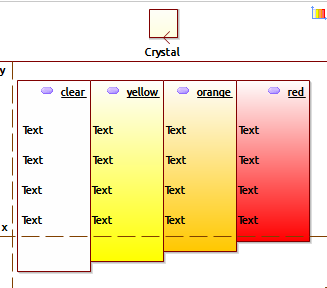
\includegraphics[width=0.7\linewidth]{proyecto/imgs/metCrystal}
	\caption{Metodoogía Ágil Crystal}
	\label{fig:metcrystal}
\end{figure}

\newpage
\subsection{Cronograma}



\begin{tabular}{|c|c|}
	\hline 
	\rule[-1ex]{0pt}{2.5ex} Hoalala & nfkfsfjd \\ 
	\hline 
	\rule[-1ex]{0pt}{2.5ex} Camila & GGuererro \\ 
	\hline 
\end{tabular} 